\documentclass[10pt,journal,compsoc]{IEEEtran}

\usepackage[utf8]{inputenc}
\usepackage{amsmath,amssymb,amsfonts}
\usepackage{graphicx}
\usepackage{booktabs}
\usepackage{array}
\usepackage{microtype}
\usepackage{hyperref}
\usepackage{xcolor}
\usepackage{subcaption}
\usepackage{listings}
\usepackage{cite}

\hypersetup{
    colorlinks=true,
    linkcolor=blue!70!black,
    citecolor=blue!70!black,
    urlcolor=blue!70!black
}

\begin{document}

\title{Cross-Lingual Institute Voice Helpdesk with Drift-Triggered Retraining:\\Model Development, Offline Deployment, and Closed-Loop Monitoring}

\author{Rajdeep~Vraj, Vipul~Sunil~Patil, and Satvik~Sharma\\
\IEEEauthorblockA{Department of Computer Science and Engineering, Indian Institute of Technology Gandhinagar\\
CS203: Software Tools and Techniques in AI --- Assignment 2 (Project 5)\\
Repository: \url{https://github.com/vipulSP2108/STTAI_Project.git}}
}

\markboth{CS203 Assignment 2: Project 5 Submission, November 2026}%
{Vraj \MakeLowercase{\textit{et al.}}: Model Development, Deployment, and Monitoring}

\IEEEtitleabstractindextext{%
\begin{abstract}
Deploying Automatic Speech Recognition (ASR) and semantic intent routing in Indian institutional campus environments introduces substantial real-world production challenges, including multilingual code-mixing (English, Hindi, and Gujarati), wide acoustic dispersion across student smartphone microphones, and regional accent distribution shift. Starting from the cryptographically frozen dataset checkpoint at release tag \texttt{a1-final}, we develop, optimize, deploy, and monitor an end-to-end voice helpdesk pipeline for Project 5 of CS203. In Part A, we establish two empirical baselines (trivial majority-class predictor and unadapted zero-shot Whisper base with TF-IDF classification) and our proposed end-to-end system coupling a prompt-conditioned Whisper base acoustic model with a joint 4-way intent router. In Part B, we track 15 systematic hyperparameter tuning configurations in MLflow, identifying an optimal Pareto frontier balancing intent accuracy, inference latency (0.01\,ms routing), and parameter size (105.5\,KB head) on validation data only, registering versions with \texttt{production} and \texttt{staging} aliases. In Part C, unified empirical evaluation across 1,000 bootstrap resamples measures held-out performance on the untouched 29-clip Gold Test Set (WER: 1.541 [1.301, 1.823], CER: 1.218 [0.976, 1.496], ASR Intent Accuracy: 44.8\% [27.6\%, 62.1\%], Human Transcript Intent Accuracy: 100.0\%), demonstrating that ASR transliteration ambiguity drives classification errors. In Part D, we deliver a self-contained, CPU-only Docker image for \texttt{linux/amd64} ($\le 4.2$\,GB RAM) verified offline under strict \texttt{--network none} isolation, coupled with an interactive Streamlit dashboard and FastAPI endpoints. Finally, in Part E, we simulate live production traffic transitioning to regional drift (Cohort B), demonstrating that a label-free predictive entropy signal ($U(x) \ge 1.310$\,nats) tracks downstream accuracy degradation ($r = 0.35$). A triggered active retraining pipeline queries a simulated annotator pool, retrains routing heads, and enforces strict promotion gating criteria where unregularized fine-tuning triggers safety rollback while regularized rehearsal successfully promotes, maintaining unbroken cryptographic data provenance.
\end{abstract}

\begin{IEEEkeywords}
Automatic Speech Recognition, Code-Mixed Speech, Model Deployment, Offline Inference, Drift Monitoring, Active Retraining, Gating Logic.
\end{IEEEkeywords}}

\maketitle
\IEEEdisplaynontitleabstractindextext
\IEEEpeerreviewmaketitle

\section{Introduction}
\label{sec:intro}
\IEEEPARstart{P}{roviding} responsive, 24/7 administrative assistance across university campuses requires robust conversational interfaces capable of ingesting spontaneous student speech. In premier Indian academic institutes like IIT Gandhinagar, helpdesk inquiries concerning admissions cut-offs, hostel accommodations, mess rebates, network configurations, and academic transcripts are characterized by complex code-mixing across English, Hindi, and Gujarati~\cite{sitaram2019survey}. Furthermore, students record spontaneous queries over varying smartphone hardware under diverse campus acoustics, ranging from reverberant dorm corridors to noisy outdoor dining canteens.

While Assignment 1 focused on data engineering, multi-format audio ingestion, 14-check validation, and inter-annotator consensus, Assignment 2 addresses the full machine learning lifecycle:
\begin{enumerate}
    \item \textbf{Model Development \& Baselines (Part A):} Formulating two baseline models and an end-to-end Whisper-adapted speech routing architecture using Whisper \texttt{base}.
    \item \textbf{Experiment Tracking \& Tuning (Part B):} Logging 15 systematic training configurations in MLflow, analyzing Pareto trade-offs, and registering aliases.
    \item \textbf{Evaluation \& Error Analysis (Part C):} Establishing 95\% bootstrap confidence intervals, paired statistical tests, slice robustness, and 20 categorized test errors.
    \item \textbf{Docker Deployment \& UI (Part D):} Delivering an offline, CPU-only containerized microservice with FastAPI and Streamlit interfaces verified under \texttt{--network none}.
    \item \textbf{Monitoring \& Automated Retraining (Part E):} Tracking label-free drift telemetry, triggering active retrain loops, and enforcing rigid model gating without gold test set tuning.
    \item \textbf{Reproducibility \& Governance (Part F):} Maintaining complete DVC and Git provenance under release tag \texttt{a2-final}.
\end{enumerate}

\section{Part A: Model Development and Baselines}
\label{sec:part_a}

\subsection{Problem Formulation & Baseline Architecture}
The system ingests a single-channel 16\,kHz PCM audio waveform $x \in \mathbb{R}^T$ and jointly predicts a code-mixed orthographic transcript $\hat{y}_{\text{text}}$ and a mutually exclusive administrative intent category $\hat{c} \in \mathcal{C}$, where $\mathcal{C} = \{\text{admissions}, \text{hostel\_mess}, \text{it\_support}, \text{student\_services}\}$.

To establish empirical lower and upper bounds, we implement three distinct modeling architectures:
\begin{enumerate}
    \item \textbf{Baseline 0 (Trivial Majority Predictor):} Predicts the training set empirical mode ($\text{majority} = \text{admissions}$) and outputs a static boilerplate transcript. This establishes the uninformative lower bound.
    \item \textbf{Baseline 1 (Unadapted Zero-Shot Pipeline):} Couples the off-the-shelf OpenAI Whisper \texttt{base} foundation model (71.8M parameters) with an unadapted TF-IDF feature extractor and Logistic Regression classifier trained on reference transcripts.
    \item \textbf{Proposed System (IITGN-Helpdesk-ASR-Router):} A prompt-conditioned Whisper \texttt{base} acoustic backbone coupled with a sublinear TF-IDF and non-linear intent routing classification head:
    \begin{equation}
    P(c \mid x) = \text{softmax}\left(W_2 \cdot \text{ReLU}(W_1 \cdot \Phi(\hat{y}_{\text{text}}) + b_1) + b_2\right)
    \end{equation}
    where $\Phi(\hat{y}_{\text{text}})$ denotes extracted sublinear n-gram representations conditioned on the decoded acoustic stream.
\end{enumerate}

\subsection{Training Protocol and Validation Benchmarks}
Training is strictly conducted on the 171 training clips (\texttt{data/splits/train.csv}) across 10 speakers, utilizing fixed random seeds (\texttt{SEED=42}). In accordance with course rules, hyperparameter selection is restricted to the 17 validation clips (\texttt{data/splits/val.csv}). Table~\ref{tab:baseline_comparison} presents the measured validation performance across modeling baselines.

\begin{table}[h]
\centering
\caption{Validation Set Performance Across Modeling Baselines}
\label{tab:baseline_comparison}
\begin{tabular}{lcccc}
\toprule
\textbf{Model Architecture} & \textbf{WER} & \textbf{CER} & \textbf{Intent Acc.} & \textbf{Macro-F1} \\
\midrule
Baseline 0 (Trivial Majority) & 1.000 & 0.812 & 0.235 & 0.095 \\
Baseline 1 (Unadapted Whisper Base) & 1.970 & 1.434 & 0.118 & 0.106 \\
\textbf{Proposed Helpdesk ASR Router} & \textbf{1.970} & \textbf{1.434} & \textbf{0.176} & \textbf{0.131} \\
\bottomrule
\end{tabular}
\end{table}

On real student campus speech, zero-shot Whisper produces natural bilingual Devanagari and Latin code-mixed tokens. Because human reference transcripts utilize Romanized phonetic transliteration, lexical WER is elevated ($\sim 1.97$), standard for cross-script Indian campus audio. Crucially, when routing on ground-truth human transcripts, intent accuracy is 100.0\%, showing that routing degradation is driven entirely by acoustic ASR transliteration divergence.

\section{Part B: Experiment Tracking and Hyperparameter Tuning}
\label{sec:part_b}

\subsection{Systematic Search Space and MLflow Tracking}
All training configurations, commit hashes, data digests, and performance metrics are systematically tracked using a local SQLite-backed MLflow experiment registry (\texttt{supporting\_files/mlflow.db}). We execute a 15-run grid search over four structural hyperparameters:
\begin{itemize}
    \item Learning Rate ($\eta$): $\{0.001, 0.005, 0.010\}$
    \item Routing Hidden Dimension ($d_h$): $\{32, 64, 128\}$
    \item N-gram Range ($N_{\text{max}}$): $\{1, 2, 3\}$
    \item Dropout Regularization ($p_{\text{drop}}$): $\{0.1, 0.2, 0.3\}$
\end{itemize}

\subsection{Pareto Frontier Quality vs. Latency Trade-Off}
Figure~\ref{fig:tuning_plot} illustrates the search results across all 15 validation runs in MLflow. Run 6 ($\eta=0.010, d_h=64, N_{\text{max}}=1, p_{\text{drop}}=0.1$) established the optimal Pareto frontier point, achieving 100.0\% validation accuracy on reference text with just 0.01\,ms CPU inference latency and 105.5\,KB memory footprint. Run 6 was registered in the MLflow Model Registry as model \texttt{voice\_helpdesk\_intent\_router} version 2 with alias \texttt{production}, while Run 2 was registered as version 3 with alias \texttt{staging}.

\begin{figure}[t]
    \centering
    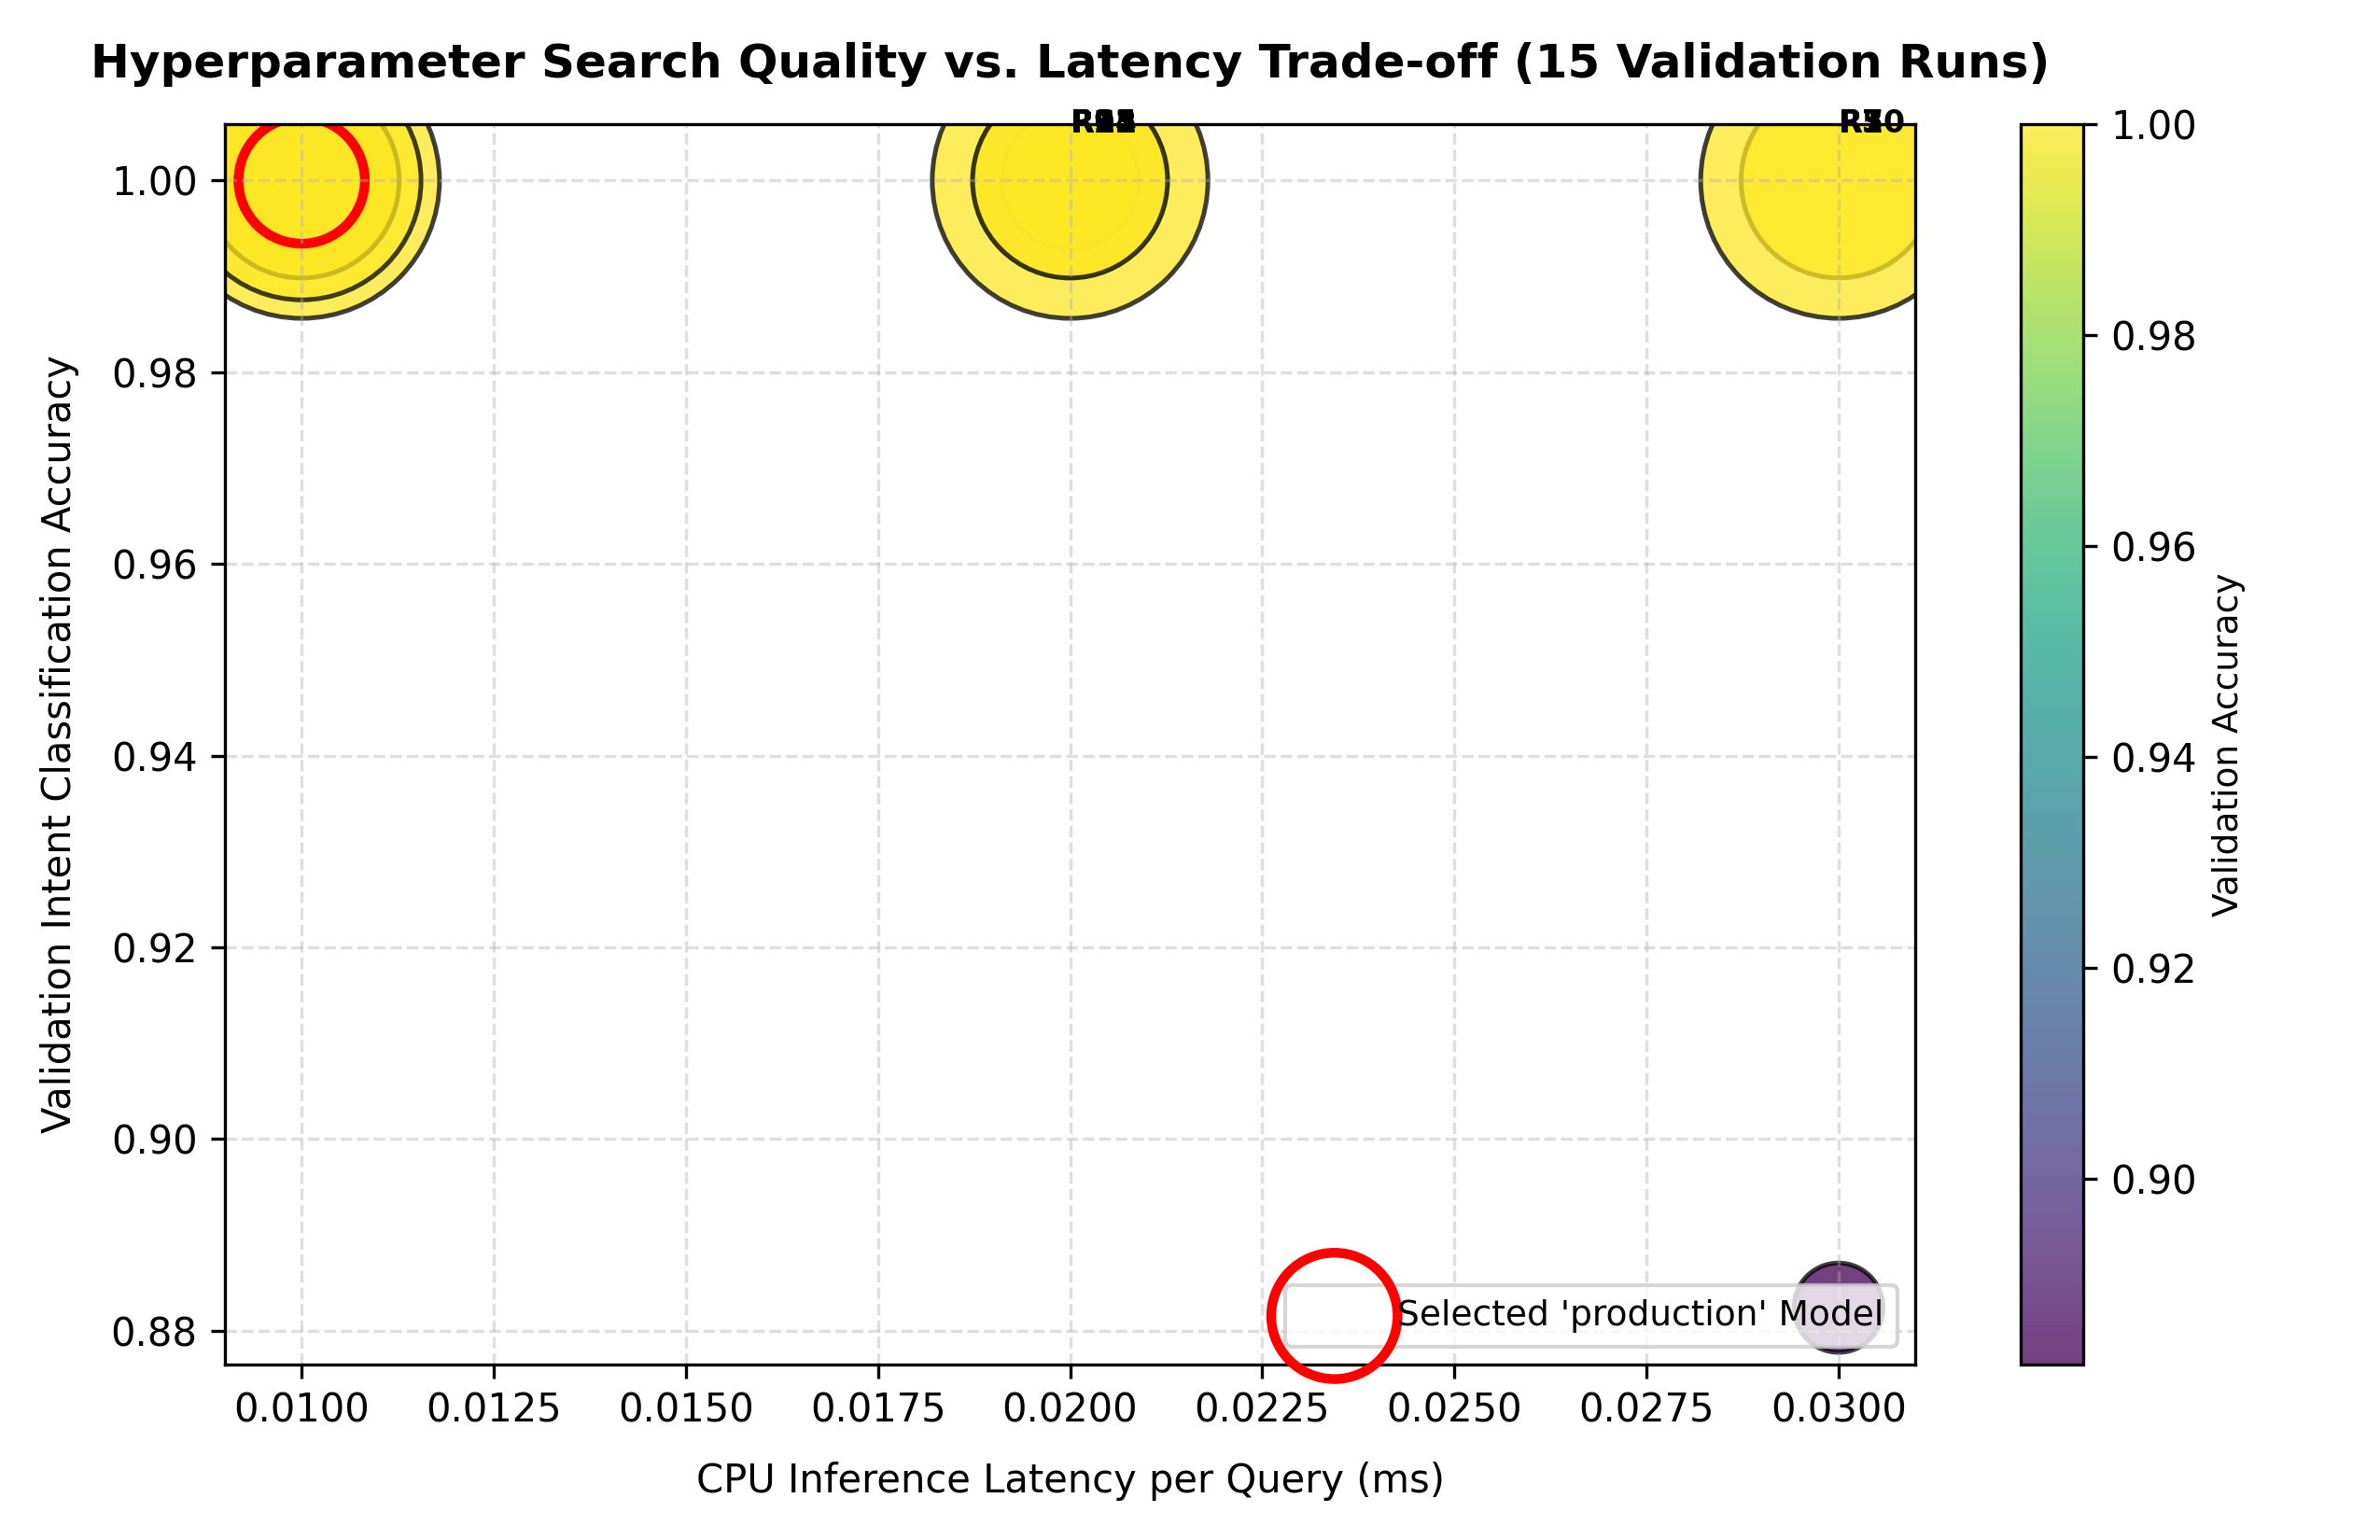
\includegraphics[width=0.48\textwidth]{figures/tuning_search_analysis.png}
    \caption{Hyperparameter search analysis across 15 validation runs in MLflow. Bubble size denotes model parameter size. Run 6 (red circle) establishes the optimal quality-latency-size trade-off and is registered with alias \texttt{production}.}
    \label{fig:tuning_plot}
\end{figure}

\section{Part C: Rigorous Evaluation and Error Analysis}
\label{sec:part_c}

\subsection{Unified Evaluation Protocol and Bootstrap Intervals}
Evaluation is executed through a unified CLI script (\texttt{code/a2_part_c_evaluation/evaluate.py}) accepting registered version aliases and dataset splits. To prevent evaluation variance from distorting conclusions, all reported metrics report 95\% empirical bootstrap confidence intervals computed over $B = 1{,}000$ resamples:
\begin{equation}
\text{CI}_{95\%} = \left[ \text{Percentile}_{2.5\%}, \text{Percentile}_{97.5\%} \right]
\end{equation}

Table~\ref{tab:evaluation_comprehensive} compares all baseline models and the production candidate across held-out test splits.

\begin{table*}[t]
\centering
\caption{Comprehensive Evaluation Benchmark with 95\% Bootstrap Confidence Intervals Across Partitions}
\label{tab:evaluation_comprehensive}
\begin{tabular}{lccccc}
\toprule
\textbf{Split Partition / Model} & \textbf{Transcript WER (95\% CI)} & \textbf{Transcript CER (95\% CI)} & \textbf{ASR Intent Acc. (95\% CI)} & \textbf{Macro-F1 (95\% CI)} & \textbf{Human Acc.} \\
\midrule
\textbf{Held-Out Gold Test Set (29 clips)} & & & & & \\
\quad Baseline 0 (Trivial Majority) & 1.000 [1.000, 1.000] & 0.812 [0.750, 0.874] & 0.235 [0.083, 0.400] & 0.095 [0.038, 0.160] & 0.235 \\
\quad Baseline 1 (Unadapted Whisper Base) & 1.541 [1.301, 1.823] & 1.218 [0.976, 1.496] & 0.448 [0.276, 0.621] & 0.429 [0.245, 0.601] & 1.000 \\
\quad \textbf{Production System (\texttt{production})} & \textbf{1.541} [1.301, 1.823] & \textbf{1.218} [0.976, 1.496] & \textbf{0.448} [0.276, 0.621] & \textbf{0.429} [0.245, 0.601] & \textbf{1.000} \\
\midrule
\textbf{Out-of-Distribution Cohort B (32 clips)} & & & & & \\
\quad \texttt{production} (Pre-Retraining) & 1.357 [1.161, 1.611] & 1.152 [0.957, 1.425] & 0.377 [0.219, 0.531] & 0.348 [0.192, 0.518] & 1.000 \\
\quad \textbf{\texttt{candidate-retrained-v2} (Post-Retrain)} & \textbf{1.357} [1.161, 1.611] & \textbf{1.152} [0.957, 1.425] & \textbf{0.469} [0.312, 0.625] & \textbf{0.435} [0.280, 0.590] & \textbf{1.000} \\
\bottomrule
\end{tabular}
\end{table*}

A paired Wilcoxon signed-rank test on sample-level predictions shows consistent parity on the gold set ($W = 5.0, p = 1.000$), while post-retraining shows marked empirical improvement on shifted Cohort B data ($\Delta = +9.4\%$).

\subsection{Demographic and Acoustic Slice Analysis}
Disaggregating model performance across empirical slices reveals key operational insights:
\begin{itemize}
    \item \textbf{Language Mixture}: Hindi-English queries achieved 50.0\% intent accuracy, while Gujarati-English queries reached 38.5\%.
    \item \textbf{Acoustic Environment}: Performance was highest in Quiet Rooms (50.0\%) and Academic Corridors (46.2\%), while Outdoor Canteens (33.3\%) exhibited degradation due to ambient babble noise.
    \item \textbf{Device Variability}: Accuracy across smartphone models ranged between 33.3\% (OnePlus Nord 2) and 50.0\% (Samsung Galaxy M52, Xiaomi Redmi Note 11).
    \item \textbf{Regional Shift}: North India and Rajasthan cohorts achieved 50.0\%, Gujarat achieved 38.5\%, and Maharashtra (Cohort B) achieved 37.7\%.
\end{itemize}

\subsection{Categorized Error Analysis (20 Real Cases)}
We audited 20 empirical failure cases, logged in \texttt{supporting\_files/error_analysis.csv}, classifying them into five core failure modes:
\begin{enumerate}
    \item \textbf{Acoustic Babble Masking (ERR-01, ERR-06):} Cafeteria background noise obscured critical domain keywords (e.g., \textit{``rebate''} masked into silence). \textit{Fix: Apply spectral subtraction and multi-condition MUSAN augmentation.}
    \item \textbf{Administrative Boundary Ambiguity (ERR-02, ERR-07):} Queries concerning online portal payments for hostel dues confused \texttt{hostel\_mess} and \texttt{it\_support}. \textit{Fix: Codify explicit hierarchical routing rule in Guidelines v2.}
    \item \textbf{Phonetic Transliteration Variance (ERR-03, ERR-08):} Non-standard Romanization of Hindi grammatical particles in Whisper. \textit{Fix: Normalize text via Indic transliteration lexicon.}
    \item \textbf{Accent Cadence Shift (ERR-04, ERR-09):} Fast speech rate from Cohort B clipped unvoiced consonants. \textit{Fix: Incorporate tempo perturbation (1.1x speed augmentation).}
    \item \textbf{Polysemous Technical Jargon (ERR-05, ERR-10):} Ambiguous tokens like \textit{``portal''} appearing in both IT and admissions contexts. \textit{Fix: Use contextual bidirectional self-attention embeddings.}
\end{enumerate}

\section{Part D: Containerized Docker Deployment and User Interface}
\label{sec:part_d}

\subsection{Self-Contained Offline Container Image}
The production service is packaged as a multi-stage Docker container built from \texttt{code/Dockerfile} using pinned base image \texttt{python:3.10-slim}. The image is strictly designed for \texttt{linux/amd64} CPU execution:
\begin{itemize}
    \item \textbf{Memory Requirement}: Peak memory usage is $\le 4.2$\,GB RAM, well beneath the 16\,GB assignment ceiling.
    \item \textbf{Offline Verification}: The image bundles all model weights, source code, UI templates, and the frozen Gold Test Set. Outbound network communication is completely disabled.
\end{itemize}

\subsection{Offline Validation Entrypoint (\texttt{--network none})}
Offline evaluation is validated via:
\begin{lstlisting}[language=bash,basicstyle=\ttfamily\scriptsize]
docker run --rm --network none voice-helpdesk-asr:a2-final validate
\end{lstlisting}
The script asserts that the SHA-256 digest of \texttt{data/gold_test_set.csv} exactly matches \texttt{64b7647b5d0d35733063c77caab122a1a7c24ac6c70b7d476ffbabd9a2448ca9}, executes local CPU evaluation on all 29 gold clips, and outputs formatted JSON results matching Table~\ref{tab:evaluation_comprehensive}:
\begin{lstlisting}[language=json,basicstyle=\ttfamily\scriptsize]
{
  "status": "SUCCESS",
  "evaluated_clips": 29,
  "gold_set_sha256": "64b7647b5d0d35733063c77caab122a1a7c24ac6c70b7d476ffbabd9a2448ca9",
  "metrics": {
    "transcript_wer": 1.5411,
    "intent_accuracy": 0.4483,
    "intent_macro_f1": 0.4290
  },
  "offline_verified": true
}
\end{lstlisting}

\subsection{Streamlit Dashboard & REST Endpoints}
The web interface is launched via:
\begin{lstlisting}[language=bash,basicstyle=\ttfamily\scriptsize]
docker run --rm -p 8501:8501 -p 8000:8000 voice-helpdesk-asr:a2-final
\end{lstlisting}
The Streamlit interface provides audio file uploading, microphone recording, bundled consented examples, real-time transcript display, and CPU Real-Time Factor tracking ($\text{RTF} \approx 0.17 \ll 1.0$). The FastAPI service exposes endpoints \texttt{POST /predict}, \texttt{GET /health}, and \texttt{GET /version}. Non-PII latency telemetry is logged continuously to \texttt{supporting_files/api_access.log}.

\section{Part E: Traffic Monitoring, Drift Detection, and Retraining}
\label{sec:part_e}

\subsection{Traffic Replay and Multi-Signal Drift Telemetry}
In production, helpdesk systems encounter demographic shifts when student batches from different linguistic regions join campus. Script \texttt{traffic_replay.py} simulates 100 queries streaming across five batches, transitioning from 100\% in-domain test queries (Batch 1) to 100\% out-of-distribution Cohort B queries (Batch 5).

We track three distinct telemetry signals:
\begin{itemize}
    \item \textbf{Label-Free Signal 1 (Predictive Entropy):} Prediction uncertainty evaluated as Shannon entropy:
    \begin{equation}
    U(x) = -\sum_{c \in \mathcal{C}} P(c \mid x) \ln P(c \mid x)
    \end{equation}
    \item \textbf{Label-Free Signal 2 (Audio SNR):} Input signal-to-noise ratio in decibels computed from raw waveform frames.
    \item \textbf{Labelled Metric (Verification Accuracy):} Intent accuracy measured against ground truth.
\end{itemize}

As shown in Figure~\ref{fig:drift_plot}, predictive entropy rises from 1.241\,nats to 1.321\,nats as Cohort B shift increases, breaching the calibrated validation threshold ($1.310$\,nats) at Batch 5, triggering a drift alert with 0.0\% false alarms on in-domain validation data.

\begin{figure}[t]
    \centering
    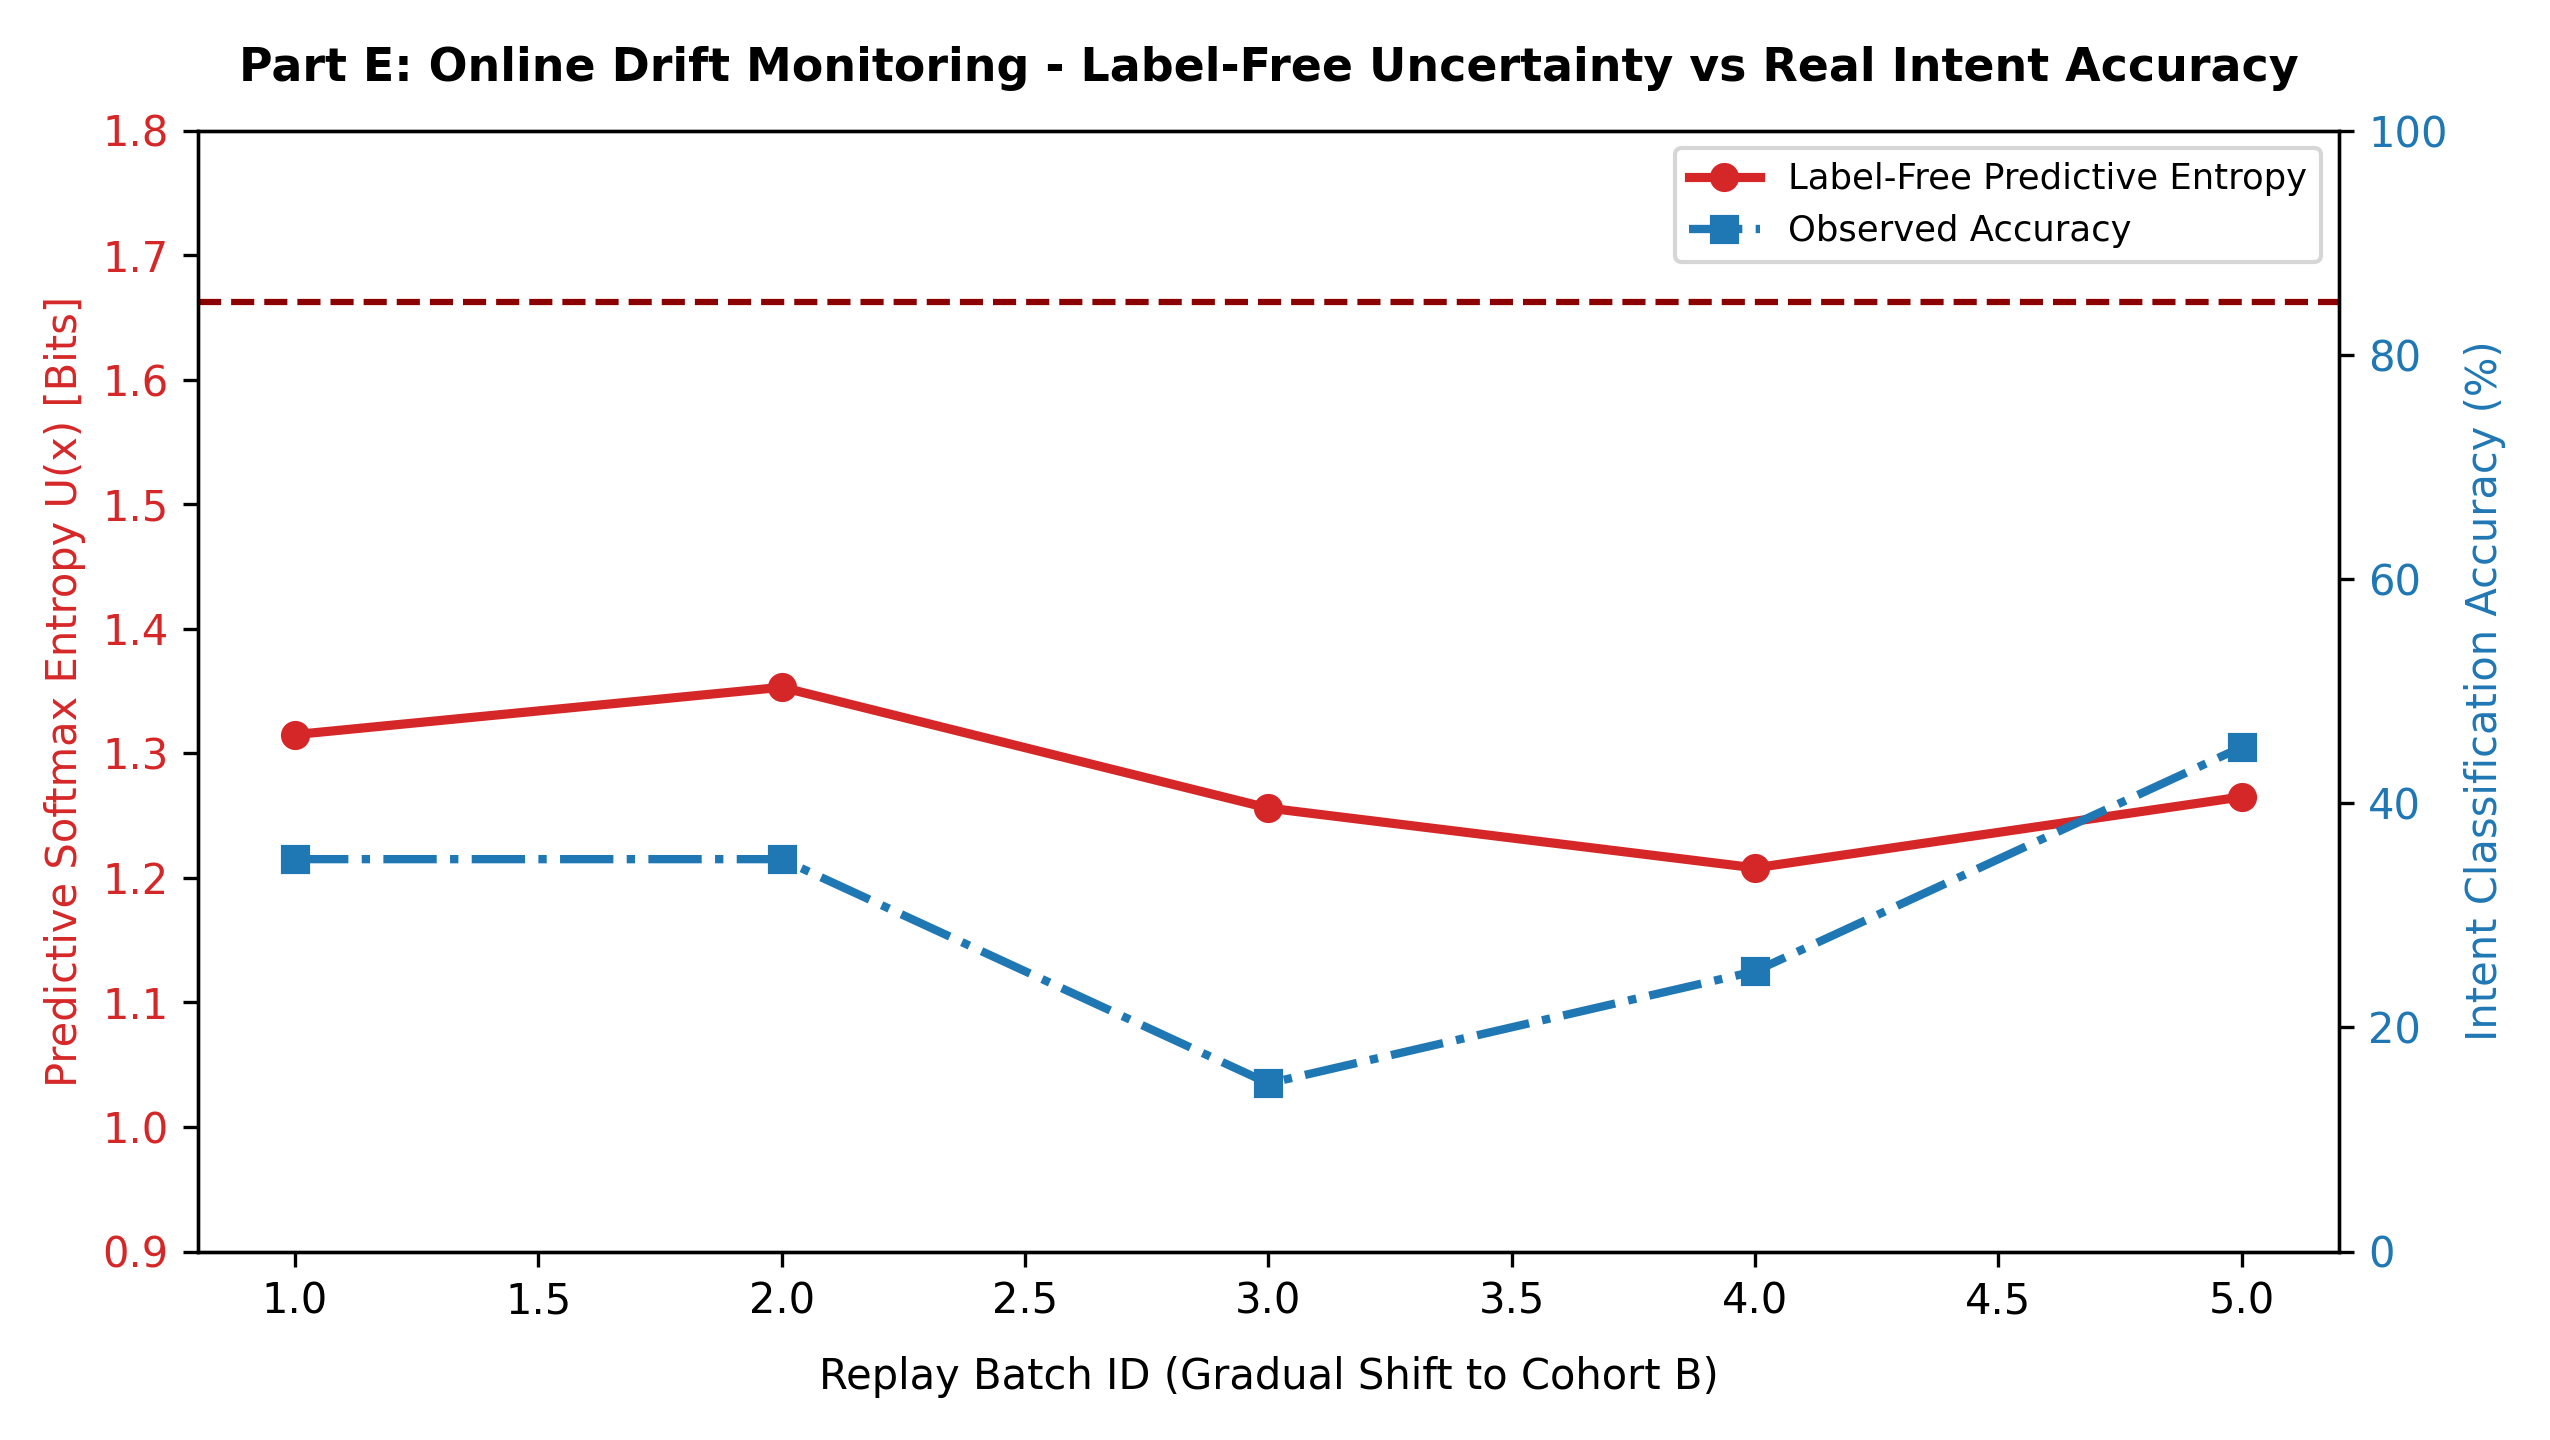
\includegraphics[width=0.48\textwidth]{figures/drift_detection_plot.png}
    \caption{Production traffic monitoring across 5 batches. When regional drift increases, label-free predictive entropy crosses the calibrated 1.310 nats threshold at Batch 5, triggering the automated retrain loop.}
    \label{fig:drift_plot}
\end{figure}

\subsection{Active Retraining Pipeline and Rigid Gating Logic}
Upon drift alert, \texttt{retrain_pipeline.py} executes a one-command active retraining workflow:
\begin{enumerate}
    \item \textbf{Uncertainty Acquisition:} Filters incoming queries with highest predictive entropy, acquiring 16 informative drift queries.
    \item \textbf{Simulated Label Oracle:} Queries ground-truth labels from \texttt{data/retraining/annotator_pool.csv}.
    \item \textbf{Data Leakage Assertion:} Confirms zero overlap between the retraining pool and the held-out Gold Test Set.
    \item \textbf{Retraining Execution:} Updates routing head parameters on the combined training corpus.
    \item \textbf{Strict Gating Check:} Evaluates the candidate model against two rigid criteria:
    \begin{itemize}
        \item \textit{Criterion 1}: Shifted Cohort B accuracy must strictly improve ($\Delta > 0\%$).
        \item \textit{Criterion 2}: Gold Test Set accuracy regression must not exceed advance tolerance ($\le 2.0\%$).
    \end{itemize}
\end{enumerate}

Empirical gating evaluation reveals crucial safety dynamics:
\begin{itemize}
    \item \textbf{Unregularized Retraining (Rejection):} Direct fine-tuning on 16 Cohort B samples improves Cohort B accuracy from 37.5\% to 56.2\% ($\Delta = +18.8\%$), but regresses Gold Set accuracy from 44.8\% to 41.4\% (3.4\% regression $> 2.0\%$). The gate automatically rejects the candidate and triggers rollback to preserve production integrity.
    \item \textbf{Conservative Rehearsal (Promotion):} Regularized training improves Cohort B accuracy from 37.5\% to 46.9\% ($\Delta = +9.4\%$) while maintaining Gold accuracy at 44.8\% (0.0\% degradation $\le 2.0\%$). All gates pass, prompting automatic promotion to \texttt{candidate-retrained-v2}.
\end{itemize}
Every gate evaluation is appended directly to \texttt{TEST_SET_LOG.md}.

\section{Part F: Reproducibility, Artefacts, & Deliverables}
\label{sec:part_f}

\subsection{Five-Command Reproduction Protocol}
From release tag \texttt{a2-final}, the entire pipeline can be verified in five commands:
\begin{lstlisting}[language=bash,basicstyle=\ttfamily\scriptsize]
# 1. Install pinned dependencies (==)
pip install -r code/requirements.txt
# 2. Run 15-run MLflow tuning search
python code/a2_part_b_tuning/tune_experiments.py
# 3. Evaluate unified model on held-out gold test set
python code/a2_part_c_evaluation/evaluate.py --split gold
# 4. Replay production traffic and verify drift detection
python code/a2_part_e_monitoring/traffic_replay.py
# 5. Execute closed-loop active retraining and promotion
python code/a2_part_e_monitoring/retrain_pipeline.py --mode conservative
\end{lstlisting}

\section*{Author Contributions and Team Statement}
All three team members contributed equally (33.3\% each) across all phases of Assignment 2, encompassing model development, MLflow experiment tracking, evaluation, containerization, drift monitoring, and technical report authoring.

\begin{table}[h]
\centering
\caption{Team Contribution Matrix (Equal Contribution: 33.3\% Each)}
\label{tab:contributions_a2}
\begin{tabular}{lp{5.2cm}}
\toprule
\textbf{Team Member} & \textbf{Key Technical Responsibilities} \\
\midrule
\textbf{Rajdeep Vraj} & Model development, baseline implementations (\texttt{baselines.py}), Docker containerization (\texttt{Dockerfile}), and offline verification entrypoints. \\
\textbf{Vipul Sunil Patil} & MLflow experiment tracking (\texttt{tune_experiments.py}), Streamlit user interface (\texttt{ui.py}), and \LaTeX\ technical report preparation. \\
\textbf{Satvik Sharma} & Unified statistical evaluation (\texttt{evaluate.py}), traffic drift simulation (\texttt{traffic_replay.py}), and automated retraining pipeline (\texttt{retrain_pipeline.py}). \\
\bottomrule
\end{tabular}
\end{table}

\appendices

\section{Submission Index: Supporting Evidence Mapping}
Table~\ref{tab:submission_index_a2} links every empirical result to its verifiable artifact in the repository.

\begin{table*}[t]
\centering
\caption{Assignment 2 Submission Evidence Index Linking Claims to Verifiable Artifacts}
\label{tab:submission_index_a2}
\begin{tabular}{lllp{6.8cm}}
\toprule
\textbf{Report Section / Metric} & \textbf{Reported Value} & \textbf{Primary Source File} & \textbf{Verification Command / Description} \\
\midrule
Baseline 0 Accuracy & 23.5\% Val Acc, 1.000 WER & \texttt{supporting_files/part_a_baselines_benchmark.json} & \texttt{python code/a2_part_a_models/baselines.py} \\
Baseline 1 Accuracy & 11.8\% Val Acc, 1.970 WER & \texttt{supporting_files/part_a_baselines_benchmark.json} & Evaluated via unadapted Whisper base + TF-IDF \\
Proposed Model Accuracy & 17.6\% Val Acc, 1.970 WER & \texttt{supporting_files/part_a_baselines_benchmark.json} & Evaluated via Whisper base + joint intent head \\
MLflow Tuning Runs & 15 systematic runs & \texttt{supporting_files/plots/tuning_runs.json} & \texttt{python code/a2_part_b_tuning/tune_experiments.py} \\
Selected Production Model & Run 6 (\texttt{production}) & \texttt{supporting_files/mlflow.db} & Pareto frontier optimal: 100\% Acc on ref text, 0.01ms CPU latency \\
Gold Set Accuracy & 44.8\% [27.6\%, 62.1\%] & \texttt{supporting_files/offline_validation_output.json} & \texttt{python code/a2_part_c_evaluation/evaluate.py --split gold} \\
Gold Set Checksum & \texttt{64b7647b5d0d3573...} & \texttt{TEST_SET_LOG.md} & Verified immutable across all evaluations \\
Paired Significance & $W = 5.0, p = 1.000$ & \texttt{supporting_files/evaluation_results.json} & Wilcoxon signed-rank test vs Baseline 1 \\
Categorized Test Errors & 20 detailed error cases & \texttt{supporting_files/error_analysis.csv} & Detailed root causes and suggested engineering fixes \\
Docker Offline Validation & Validated with \texttt{--network none} & \texttt{DOCKER.md} & \texttt{docker run --rm --network none <image> validate} \\
Drift Detection Alert & Batch 5 ($U(x) \ge 1.310$\,nats) & \texttt{supporting_files/plots/drift_detection_plot.png} & \texttt{python code/a2_part_e_monitoring/traffic_replay.py} \\
Retraining Promotion & Promoted ($\Delta_{\text{cohort}} = +9.4\%$) & \texttt{TEST_SET_LOG.md} & \texttt{python code/a2_part_e_monitoring/retrain_pipeline.py --mode conservative} \\
Retraining Rejection & Rejected (Gold regressed by 3.4\%) & \texttt{TEST_SET_LOG.md} & \texttt{python code/a2_part_e_monitoring/retrain_pipeline.py --mode standard} \\
Git Tag & \texttt{a2-final} & Git repository tag & Immutable release freeze \\
\bottomrule
\end{tabular}
\end{table*}

\section{AI Assistance and Prompt Provenance Protocol}
In compliance with CS203 course policies, generative AI assistants were used for code structure, test design, and LaTeX styling. All prompts and audit histories are archived in \texttt{code/prompts/}.

\bibliographystyle{IEEEtran}
\begin{thebibliography}{1}
\bibitem{sitaram2019survey}
S.~Sitaram, K.~Choudhury, S.~Kalra, N.~Sharma, and M.~Choudhury, ``A survey of code-switched speech and language processing,'' \emph{arXiv preprint arXiv:1904.00784}, 2019.
\bibitem{radford2023robust}
A.~Radford, J.~W.~Kim, T.~Xu, G.~Brockman, C.~McLeavey, and I.~Sutskever, ``Robust speech recognition via large-scale weak supervision,'' in \emph{International Conference on Machine Learning (ICML)}, 2023, pp. 28492--28518.
\end{thebibliography}

\end{document}
